\documentclass{article}
\usepackage{geometry} 
\geometry{letterpaper} 
%%%% Uncomment below to begin paragraphs with an empty line %%%%
\usepackage[parfill]{parskip} 
\usepackage{graphicx}
\usepackage{amssymb}
\usepackage{moreverb}
%\usepackage[section]{placeins}
%\usepackage[below]{placeins}
\usepackage{epstopdf}
%\DeclareGraphicsRule{.tif}{png}{.png}{`convert #1 `dirname #1`/`basename #1 .tif`.png}
\newcommand\bslash{\char`\\}
\newcommand\lt{\char`\<}
\newcommand\gt{\char`\>}
\newcommand{\tab}{\hspace*{2em}}
\newcommand{\supers}[1]{\ensuremath{^\textrm{{\scriptsize #1}}}}
\newcommand{\subs}[1]{\ensuremath{_\textrm{{\scriptsize #1}}}}
\newcommand{\notebox}[1]{ \begin{center}\framebox[5.5in]{\begin{minipage}[t]{5.0in}\textbf{Note: }#1\end{minipage}}\end{center}}

\title{Transient Component Simulator Reference}
\author{Aron P. Dobos}

\begin{document}

\maketitle
\vspace{3in}
\begin{abstract}
The Transient Component Simulator (TCS) software package is an integrated system for performing transient analysis of physical systems.  It is designed for use in multi-threaded and embedded environments, including the System Advisor Model (SAM) tool developed by the National Renewable Energy Laboratory.  It is comprised of an iterative solver kernel that can dynamically load system component libraries, each of which can define one or more component descriptions.  Each component is a unique type that defines its inputs and outputs, and the associated calculations.  The TCS package also includes a simple graphical system editor in which the user can define connections between components, as well as a scripting interface (using the LK script engine), a timeseries graph viewer, and a tabular data browser.

The TCS kernel is designed to be fully reentrant and thread-safe, and is written in ISO-standard C++, allowing it to be highly portable across a variety of host platforms.
\end{abstract} 

\newpage
\tableofcontents
%%\listoffigures
%%\listoftables
\newpage

\section{Overview}

The Transient Component Simulator (TCS) is a general purpose transient physical system simulation tool at whose core is an iterative successive-substitution solving engine.  Each unique physical system component is known as a \emph{type}, and instances of types are \emph{units}.  A system consists of a set of \emph{n} units ordered 0..\emph{n}-1.  It is allowed to have multiple units of the same type in a system.  The order in which units are defined in the system is the same order that the iterative solver calls each type at each timestep.  A type is essentially a compiled subroutine that calculates the values of output variables from input variables.

Each type defines a specific set of input and output variables.  Each variable is given at compile-time a data type, index, label, units, description, optional metadata, and optional default value.  Variables can be numbers, one dimensional arrays, two dimensional matrices, or strings.  There is no defined limit on the number of variables, or size of arrays and matrices.  Information about a type's input and output variables can be dynamically queried through the TCS application programming interface (API).  More details on variables and data types will be given in Section~\ref{sec_types}.

A simulation progresses with a constant time step from a specified start time to a specified end time.  The internal time unit in TCS is the \emph{second}, although for convenience the default user interface allows time specification in hours.  At each time step, TCS calls each unit in the given calling sequence.  After each unit is called, TCS checks to see if any of the outputs are connected to inputs of other units.  If so, TCS propagates the output value to the input value, marking the unit associated with the input for iteration if the previous input value was outside the specified tolerance for the particular connection.  TCS repeats the unit calling sequence, calling only marked units until all output and input values have converged to tolerances and there are no marked units left in the calling sequence.  At this point, the simulation is said to have converged at that timestep.  TCS increments the time and repeats this sequence at the next time step until the end time is reached.

Key features of the simulator kernel include:
\begin{itemize}
\item Fully dynamic type interface API:  Types can be written in C or C++, and dynamically loaded by the TCS kernel.  Because the type API uses the standard C \texttt{\_\_cdecl} calling convention, types can be written using any standard C or C++ compiler.
\item Multithreading: The TCS kernel is fully reentrant and thread-safe, allowing it work well with host software that can dispatch concurrent simulations, provided all the types used in a simulation are also written in this way.
\item Data types:  Input and output variables can be numbers, arrays, matrics, or strings.  This affords significant flexibility when defining a type subroutine and moving data between units.
\end{itemize}

The TCS Simulator Console has five main parts:
\begin{itemize}
\item \textbf{Visual Editor}: The visual editor allows the user to create instances of types (called units), and connect outputs to inputs by drawing lines between components.  Units can be added, deleted, and reordered.  Connections can be added, deleted, re-routed, and configured to have unique tolerances associated with them.
\item \textbf{Script Editor}: The script editor allows the user to programmatically configure a system, run a simulation, and extract results.  Using looping constructs, parametric analyses could be constructed to analyze a design across various input parameters.  The LK script language runs fast and is simple to use, and includes a large standard library of built-in functions for working with files, strings, mathematics, and basic user interface interactions.
\item \textbf{Timeseries Graphs}: The timeseries data viewer implements a full-featured visualization component based on DView to observe numeric data variables at each timestep of the simulation.  Plots include time series, heat maps, scatter plots, day and month averages, CDF and PDF statistical distributions, and duration curves.
\item \textbf{Data Tables}: The data tables make all input and output variable values available in a tabular data grid that can quickly load and display the large time-series datasets generated by a transient simulation.
\item \textbf{Messages Window}: At the bottom of the TCS application, a log window displays messages and information generated by various actions in the user interface.
\end{itemize}

A screenshot of the TCS console application is included in Figure~\ref{fig_tcsconsole}.

\begin{figure}[hp]
\begin{center}\scalebox{0.65}{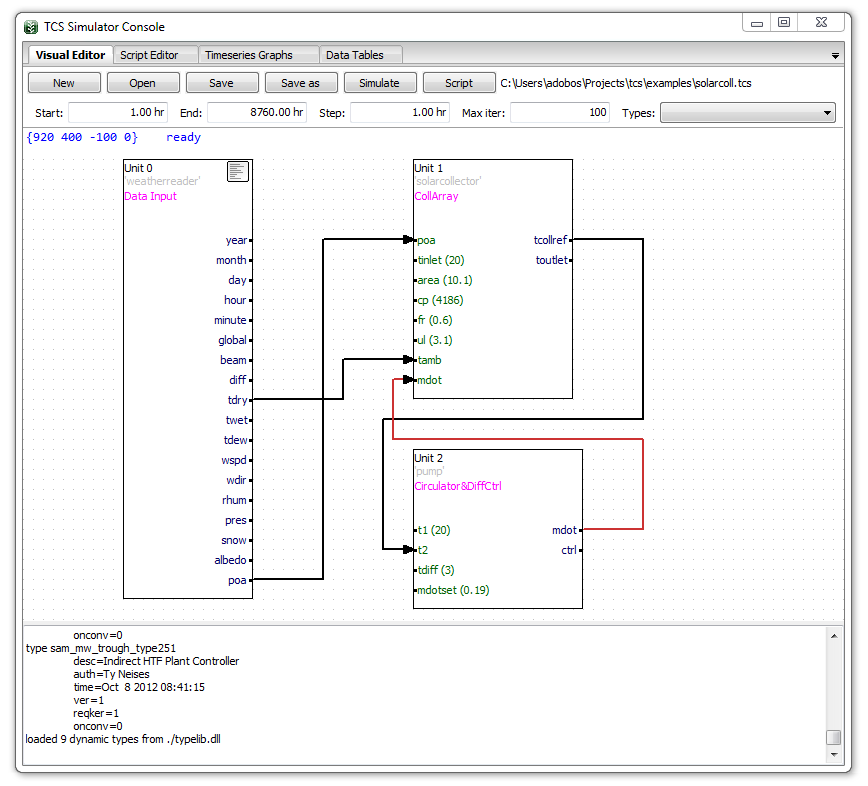
\includegraphics{tcs_console.png}}\end{center}
\caption{TCS Simulator Console screenshot showing a system in the visual editor.}
\label{fig_tcsconsole}
\end{figure}


\section{Getting Started}
\subsection{Required Tools}

\textbf{Note:} \emph{In November 2012 or thereabouts, we plan to upgrade TCS and associated software libraries to use Visual Studio 2012 Express.  These instructions will be updated accordingly at that time.}
\vspace{0.25in}

For Windows platforms, TCS is developed using Microsoft Visual C++ 2010 Express Edition.  Download the installer from:\\
\texttt{http://www.microsoft.com/visualstudio/en-us/products/2010-editions/visual-cpp-express}\\ and run it.  After installation, you will need to register on the Microsoft website to obtain a free registration code that will enable VC++ 2010 to run past 30 days.

You also will need Microsoft Visual C++ 2008 Express Edition to convert the wxWidgets project files properly.  Download from:\\
\texttt{http://www.microsoft.com/visualstudio/en-us/products/2008-editions/express}\\No registration code is required for the 2008 version.

The default TCS user interface requires also the wxWidgets 2.8.12 library.  Download the Windows (MSW) \texttt{.zip} version of it from:\\ \texttt{http://prdownloads.sourceforge.net/wxwindows/wxMSW-2.8.12.zip}\\
Unzip the file to \texttt{c:\bslash wxMSW-2.8.12-vc2010}.
\\\\
To compile wxWidgets 2.8.12, follow these steps:
\begin{enumerate}
\item Start Visual C++ 2008 Express.
\item Open \texttt{c:\bslash wxMSW-2.8.12-vc2010\bslash build\bslash msw\bslash wx.dsw} and allow all the projects to be upgraded.
\item Click \texttt{Save All} to save the upgraded solution and project files.
\item Repeat the previous two steps for \texttt{contrib\bslash build\bslash stc\bslash stc.dsw} and \texttt{contrib\bslash build\bslash net\bslash net.dsw}
\item Close Visual C++ 2008, and open Visual C++ 2010.
\item Open \texttt{c:\bslash wxMSW-2.8.12-vc2010\bslash build\bslash msw\bslash wx.sln}, and allow the whole solution and all projects to be upgraded to the latest Visual C++ version.
\item Once the project conversion is complete (this can take some time), click \texttt{Save All}
\item Right click in the solution explorer on 'wx', and select \texttt{Batch Build...}.  Check all of the \texttt{Debug} and \texttt{Release} configurations, and click \texttt{Build}.  Wait for all 40 projects to be built.
\item Open \texttt{contrib\bslash build\bslash stc\bslash stc.sln} and allow the project to be converted.  Right click on the solution and choose \texttt{Batch Build...}, and check the \texttt{Debug} and \texttt{Release} builds, and click \texttt{Build}.
\item Repeat the previous step for  \texttt{contrib\bslash build\bslash net\bslash net.sln}
\end{enumerate}
At this point, the wxWidgets 2.8.12 libraries should be successfully compiled with Visual C++ 2010.

\subsection{Checking Out}
The TCS source code is stored on the \texttt{efmsvn.nrel.gov} Subversion server hosted by NREL IS.  Use your NREL network username and password when prompted for access credentials.  On Windows, use the TortoiseSVN subversion client, downloadable from:\\
\texttt{http://tortoisesvn.net/downloads.html}
\\Follow the steps below to obtain the various projects need for TCS:
\begin{enumerate}
\item Create a new folder, for example \texttt{c:\bslash Projects}. In your new project folder, create the following subfolders: \texttt{comlib}, \texttt{lk}, \texttt{ssc}, \texttt{tcs}
\item Right click on \texttt{comlib}, and select \texttt{SVN Checkout...}.  In the checkout window, enter the URL\\
\texttt{https://efmsvn.nrel.gov/comlib/svn/trunk} and click OK.

\item Right click on \texttt{lk}, and select \texttt{SVN Checkout...}. In the checkout window, enter the URL\\
\texttt{https://efmsvn.nrel.gov/lk/svn} and click OK.

\item Right click on \texttt{ssc}, and select \texttt{SVN Checkout...}. In the checkout window, enter the URL\\
\texttt{https://efmsvn.nrel.gov/ssc/svn/trunk} and click OK.

\item Right click on \texttt{tcs}, and select \texttt{SVN Checkout...}. In the checkout window, enter the URL\\
\texttt{https://efmsvn.nrel.gov/tcs/svn} and click OK.
\end{enumerate}
All of the required source code for TCS and the supporting libraries should be locally available now.

\subsection{Environment Variables}
Several environment variables must be configured for Visual C++ to correctly locate the various projects. To set an environment variable, go to Start$\rightarrow$Control Panel$\rightarrow$System$\rightarrow$Advanced system settings$\rightarrow$Environment variables.
\begin{enumerate}
\item CMLMSW = \texttt{c:\bslash Projects\bslash comlib}
\item LKDIR = \texttt{c:\bslash Projects\bslash lk}
\item SSCDIR = \texttt{c:\bslash Projects\bslash ssc}
\item WXMSW = \texttt{c:\bslash wxMSW-2.8.12-vc2010}
\end{enumerate}

\subsection{Compiling and Running}

The \texttt{comlib} project contain extra wxWidgets user interface controls and utility functions that the TCS user interface requires for graphing and data tables.  \texttt{SSC} is the core simulator interface used by SAM and other NREL web services, and contains a sub-library \texttt{recore} that contains numerous useful energy modeling and related subroutines that are helpful for composing new TCS component models.

\begin{enumerate}
\item Open \texttt{c:\bslash Projects\bslash comlib\bslash comlib.sln} in Visual C++ 2010.  Build both \texttt{Debug} and \texttt{Release} targets.
\item Open \texttt{c:\bslash Projects\bslash lk\bslash vc\_build\bslash lk.sln} and batch build \texttt{Debug} and \texttt{Release} targets.
\item Open \texttt{c:\bslash Projects\bslash ssc\bslash ssc.sln} and batch build all \texttt{Debug} and \texttt{Release} targets.
\item Open \texttt{c:\bslash Projects\bslash tcs\bslash tcs.sln} and batch build all \texttt{Debug} and \texttt{Release} targets.
\end{enumerate}

When all of these projects have successfully compiled, run the TCS 'main' project.  You should see a graphical user interface pop up with the title 'TCS Simulator Console'.

\section{Visual Editor}

The visual editor in the TCS console provides a graphical method for defining a physical system.  All editing actions are initiated from a right-click context menu that changes depending on the state of the editor.  There is also a status bar that displays information including display coordinates, information about variables and units, and current actions.

\subsection{Navigation}
The editor is navigated by a combination of keyboard and mouse maneuvers.  Important keyboard actions are listed below.
\begin{itemize}
\item \texttt{Left Arrow}:  Scrolls the display to the left.
\item \texttt{Right Arrow}:  Scrolls the display to the right.
\item \texttt{Up Arrow}:  Scrolls the display upwards.
\item \texttt{Down Arrow}:  Scrolls the display downwards.
\item \texttt{Escape}: Cancels any pending action, including \emph{move} and \emph{connect} operations.
\end{itemize}

\subsection{Working With Units}

To create a new unit, right click on the gridded canvas, and choose from the available types that are listed in the popup menu.  A rectangular box will appear on the layout with all input variables listed on the left side and all the output variables on the right side.  The unit number (simulation order) will appear at the top, followed by the unit's type, and an optional description.  To delete a unit, right click on it, and choose \emph{Delete unit} from the menu.  A unit can be moved around the screen by left-clicking, holding, and dragging the unit.  A rubber-band outline of the unit will appear as it is being moved.


When there are several units in a system, it is possible to change the simulation order.  Right click on a unit, and selected either \emph{Move up (order)} or \emph{Move down (order)}.  Moving a unit up swaps it with the previous unit in the simulation order, and so repeatedly moving a unit up will eventually make it the first unit in the simulation (Unit 0).  Moving a unit down performs the same operation in the opposite direction.

Units can be assigned a description, parameter values, as well as initial values for inputs.  To show the unit values dialog, either double-click with the left mouse button on a unit, or choose \emph{Edit unit values...} in the context menu.  A dialog will appear in which you can enter a description, and a multi-line text entry for input variable values.  The dialog also shows a table with all of the unit's input and output variables for reference.  The dialog is shown in Figure~\ref{fig_editunit}.

\begin{figure}[hp]
\begin{center}\scalebox{0.75}{\includegraphics{edit_unit.png}}\end{center}
\caption{Unit properties dialog.}
\label{fig_editunit}
\end{figure}

To assign values to example variables \emph{file\_name}, \emph{tilt}, \emph{temperatures}, \emph{fluxmap}, use the example syntax listed below.

\begin{verbatim}
file_name=C:/Weather Data/TX Abilene.tm2
tilt=30.52
temperatures=-1.2,0.5,1.6,1.9,2.3,4.5,9.6
fluxmap=[1,0,0][0,1,0][0,0,1]
\end{verbatim}

This shows how to assign values to variables of string, number, array, and matrix data types.  Click \emph{OK} on the \emph{Edit values} dialog to accept the changes.  Numeric values will be shown on the unit display, and other variables that were given values are also updated to green from red.  The color of an input variable label indicates whether or not it is connected or has been assigned an initial value.  Green indicates that the input has an explicit value or is fed by an connection from an output, while red means that the variable is unassigned and may default to any internally set default value or unknown value.  

\notebox{By default, TCS will load the \texttt{typelib.dll} library of types that is part of the overall TCS Visual C++ solution.  Future versions of TCS console will allow other dynamic type libraries to be loaded as well. }

\subsection{Parameters, Inputs, Outputs, and Debug Variables}

A type may define some inputs as parameters, and some outputs as debug values.  A parameter is treated exactly the same as an input variable inside the simulator kernel.  The purpose of defining a variable as a parameter is to emphasize that its value should not change over the course of the simulation, and also to hide the variable from the left side of automatically generated graphical unit that is shown in the visual editor.  A parameter is assigned a value in the \emph{Edit unit values} dialog, in the same way as a normal input variable.  An unassigned numeric parameter by default is given a value of 0.0.

A debug variable is treated exactly the same way as a normal output variable inside the TCS kernel.  The only difference is that it is not shown along with the other outputs of a unit in the visual editor, and that its value cannot be connected to another unit's input.  The purpose is to allow for units to provide additional debugging information during simulation without cluttering the intended core outputs of the type.


\subsection{Making Connections}

Connections are made from outputs to inputs.  Only one output can be assigned to a particular input, but any output can feed multiple different inputs.  To make a connection, move the mouse cursor over the black dot at an output variable, and when the cursor changes to a bullseye, click with the left mouse button.  A thin wire will be drawn, and the status bar will change to \emph{connecting}.  Draw the wire in the direction of the target input, clicking as you go to place \emph{waypoints} to make the drawing look nice.  The wire coordinates will automatically snap to the default grid.  To finish a connection, choose the unconnected input variable, and hover over it until the bullseye cursor appears and the status bar asks \emph{finish connection here?}.  Click with the left mouse button to make the connection, and the wire will darken and an arrow will be drawn to shown the direction of information flow in the system.  If the output and input variables have particular units defined for the data, the editor will draw the wire in orange if the units do not match.  To cancel a connection before it has been attached to an input, press the \emph{Escape} key.

Often it is helpful to move waypoints along a wire to improve the drawing.  Hover over a waypoint until the pencil cursor appears, then left-click and drag the waypoint to another spot.  When you release the left mouse button, the wire will be redrawn.  To edit a connection path, you can add a waypoint near another, or delete a waypoint.  Hover over an existing waypoint until the pencil cursor appears, right-click, and choose the appropriate action from the popup menu.

To delete a connection, right click on a waypoint and choose \emph{Delete connection}.  Or you can right click on an input or output variable, and choose \emph{Delete all connections at this point}.  For an output variable that feeds multiple inputs, choosing this action will delete all of those connections at once.  Deleting a unit will also delete any connections to and from that unit.

To edit a connection's properties, right-click on a waypoint and choose \emph{Edit connection}, and a dialog will shown.  The dialog allowing you to enter a specific tolerance for the particular connection, and an array index if applicable.  The default tolerance is 0.1 \%.  Entering a positive number means that the value is interpreted as a relative tolerance specified as a percentage.  Negative numbers are interpreted as the maximum absolute difference between the output and input.  For example, entering -0.5 means that the input and output must converge to less than 0.5 of one another, regardless of the units.  For connections that connect an \emph{array} output to a \emph{number} input, you must specify the index of the output array to propagate to the input.  Arrays are indexed starting at 0.  If the array index specified in a connection is greater than the length of the array during simulation, an error will be issued and the simulation will stop.

\subsection{Files and Exports}

The visual editor saves the system layout in a proprietary binary file format with the extension \texttt{.tcs}.  The format is relatively straightforward and efficient.

To export an image of the entire physical system layout as shown in the visual editor, right click and choose \emph{Copy view to clipboard (image)}.  This place a bitmap image of the layout on the clipboard that can be pasted into other applications.  The grid and statusbar are not shown in the exported image, and the image is cropped to the extents of the system layout.

\subsection{Running Simulations}

To run a simulation, press the \emph{Simulate} button on the top toolbar.  Enter the start time, end time, and time step in hours.  Note that the internal simulation time is represented in seconds, but hours are used in the interface for ease of use.  By default, the simulation is configured to run from hours 1 to 8760 (one year) at one hour timesteps.

When the \emph{Simulate} button is clicked, the visual editor will generate a \emph{netlist} that lists all of the units in the calling sequencer and all of the connections drawn on the layout.  The netlist will be displayed in the messages window at the bottom of the screen, and the system representation will be loaded into the TCS simulation kernel. A progress dialog will appear to show the progress of the simulation.

As the simulation progresses, the values of all input and output variables for each unit are automatically saved in memory at the end of each time step when convergence has been achieved.  When the simulation is complete, the results are made available in the timeseries graph viewer and the data table grid.

\section{Script Editor}

The scripting capability in the TCS console operates as a separate way to control the simulation kernel.  The TCS Console uses the LK ('language kit') scripting language engine and is fully integrated into the interface.  Separate reference documentation is available that describes the language in detail. 

\subsection{Capabilities}

Scripting allows for:
\begin{itemize}
\item Setting up complex systems that could be cumbersome to visually lay out
\item Programmatically generate system designs
\item Working with external files in other formats that describe a system
\item Performing parametric simulations that adjust system parameters over a range
\item Post-processing on outputs for validation and calculating metrics
\item Exporting customized datasets from a simulation to files
\end{itemize}

The standard library of built-in scripting functions includes extensive capabilities for mathematics, string and data processing, file input and output, and graphical 2-D plotting functions.  See the example scripts in the TCS \texttt{examples/} folder for examples on more advanced scripting techniques.

\subsection{Editing Scripts}

The script editor can edit one script file at a time.  Scripts are saved as text files with the \texttt{.lk} extension.  The editor performs syntax highlighting for the LK language, provides calltip information for function calls while typing, and has enhanced indentation to help organize script code.  A basic Find \& Replace dialog allows for searching the text.  Clicking on the \emph{Help} button will pop up documentation for all of the built-in functions calls in the LK standard library that are available to the user.

\subsection{Running a Script}

To execute the script code, press the \emph{Run} button on the top toolbar.  If there are any syntax errors, they will be listed in the messages window and script processing will stop.  If the syntax is legal, the script will be executed in a clean environment.  This means that any variables created in previous executions of the script are not saved and each time the script is running in a clean slate.  At the beginning of a run, the messages window is cleared, and the start time is displayed.  When the script has finished executing, the elapsed time for the entire script execution is displayed in the window.

For example, the script below will request input from the user and then display the response several times.

\begin{verbatim}
x = in();
for (i=0;i<4;i++) outln(x+x);
\end{verbatim}

Running the script and entering \texttt{abc} at the prompt will generate output something like:

\begin{verbatim}
Start: Fri Jan 06 14:44:06 2012
abcabc
abcabc
abcabc
abcabc
elapsed time: 2197 msec
\end{verbatim}

\subsection{TCS-specific Functions}

\texttt{clear (none):string}\\
Clear all units and connections.
\\\\
\texttt{add\_unit (string:type name, [string:description]):integer}\\
Add a unit to the simulator. 
\\\\
\texttt{set\_value (integer:unit, string:variable name, any:value):void}\\
Set a variable value for a unit. Values can be a number, string, array, or 2D array. 
\\\\
\texttt{connect (integer:unit1, string:output name, integer:unit2, string:input name,
[number:ftol=0.1], [number:arridx=-1]):boolean}\\
Make a connection from an output to an input. 
\\\\
\texttt{simulate (number:start, number:end, number:step, [number:maxiter=100]):number}\\
Run a simulation in the given time range specified in hours. 
\\\\
\texttt{netlist (void):string}\\
Generate a netlist description of the current configuration. 
\\\\
\texttt{get\_result (integer:unit, string:variable name):array}\\
Obtain the values of for a particular variable at all timesteps after a simulation. 

\section{Graph Viewer}

The graph viewer uses the \emph{wxDView} library (included in \texttt{comlib}) and includes time series, heat map, monthly, scatter, PDF/CDF, and duration curve plots.  During simulation, the values of each numeric input and output variable for each unit are saved at each time step.  When the simulation is complete, the data is rendered in all of the viewer graphs with the correct time step and start time offset.  The viewer can accommodates subhourly data as well as sequences longer than one year (8760 hours).  

The view perspective is saved before a new simulation starts and is re-applied when it is finished.  The same time period will be shown of the same checked variables, making it straightforward to compare results after making a change to the system.

\section{Tabular Results}

The tabular data browser provides access to all of the input and output variables of all units (of all data types) after a simulation.  Use the check list box to add and remove variables from the data table.  Columns can be resized to better accommodate the data shown.  The view is refreshed automatically after re-running a simulation.


\section{Writing Types}\label{sec_types}

Types are compiled software subroutines that describe a physical system component in TCS.  While the interaction with the TCS kernel is achieved through a purely C language (using the \texttt{\_\_cdecl} calling convention) interface, we expect most type writers will use the provided C++ wrapper to facilitate easy structuring of the necessary codes.  The entire interface and C++ wrapper is defined inline in the \texttt{tcstype.h} header file provided with the TCS distribution.  This it the only file that needs to be distributed to and included by people writing types for the TCS kernel - no other special linkages or libraries are needed.

\subsection{Type Structure}

Writing a type is best explained by observing an example in detail.  Here we present the implementation of a simple pump and controller that produces a constant volumetric flow rate if the upper input temperature is greater than the lower input temperature by the set difference threshold.  The type is implemented in C++ using the TCS standard wrapper interface in \texttt{tcstype.h}.


In this example, the pump and controller will be compiled as a single type in one dynamic library that can be loaded by the TCS kernel.  The listing below can be entered into \texttt{pump.cpp} and compiled independently of all other types, if desired.


At the top of source file implementing a type, include the two lines below.  The \texttt{\_TCSTYPEINTERFACE\_} macro enables code in the \texttt{tcstype.h} header file used for writing types.

\begin{verbatimtab}[4]
#define _TCSTYPEINTERFACE_
#include "tcstype.h"

\end{verbatimtab}

The next section defines the variable types, indexes, names, labels, units, group name, meta data, and default values for each parameter, input, output or debug variable.  First, an \emph{enumeration} lists all of the input and output variables.  This enumeration generates named indices that will make it easy and fast to access variables in the middle of a simulation. \textbf{It is essential that the order of variables in the enumeration and the subsequent table is the same.}  It is suggested that parameters begin with \texttt{P\_}, inputs begin with \texttt{I\_}, outputs with \texttt{O\_} and debug variables with \texttt{D\_} for clarity, and that they are declared in the order: parameters, inputs, outputs, and debug variables.  Each row in the \texttt{tcsvarinfo} table defines one variable.  The various fields specified in each row are the fields in the C structure
\begin{center}
\begin{boxedverbatim}
struct _tcsvarinfo {
  unsigned char var_type; // TCS_PARAM, TCS_INPUT, TCS_OUTPUT, TCS_DEBUG
  unsigned char data_type; // TCS_NUMBER, TCS_ARRAY, TCS_MATRIX, TCS_STRING
  unsigned int index;
  const char *name;
  const char *label;
  const char *units;
  const char *group;
  const char *meta;
  const char *default_value;
}
\end{boxedverbatim}
\end{center}

The enumeration and variable table defining the two parameters, two input variables and two output variables for the pump/ controller are shown below.

\begin{verbatimtab}[4]
enum {	P_MDOTSET,
        P_TDIFF,

        I_T1,
		I_T2,

		O_MDOT,
		O_CTRL,

		N_MAX };

tcsvarinfo pump_variables[] = {

{ TCS_PARAM, TCS_NUMBER,   I_MDOTSET, "mdotset", "Design flow rate",    "L/s", "", "", "" },
{ TCS_PARAM, TCS_NUMBER,   I_TDIFF,   "tdiff",   "Difference setpoint", "'C",  "", "", "" },

{ TCS_INPUT, TCS_NUMBER,   I_T1,      "t1",      "Test temperature 1",  "'C",  "", "", "" },
{ TCS_INPUT, TCS_NUMBER,   I_T2,      "t2",      "Test temperature 2",  "'C",  "", "", "" },

{ TCS_OUTPUT, TCS_NUMBER,  O_MDOT,    "mdot",    "Flow rate",           "L/s", "", "", "" },
{ TCS_OUTPUT, TCS_NUMBER,  O_CTRL,    "ctrl",    "Control signal",      "0/1", "", "", "" },
	
{ TCS_INVALID, TCS_INVALID,  N_MAX,   0,         0, 0, 0, 0, 0 } };


\end{verbatimtab}
The next section defines a new C++ \emph{class} that implements the type.  Each unit in the TCS kernel is an instance of the type's class defined below.  That is, all member variables of the class are unique to each instance of the type, meaning that multiple instances of the same type will not overwrite each other's data variables.  \textbf{It is important to avoid using \texttt{static} or global variables in types.}  The \texttt{pump} class extends the \texttt{tcstypeinterface} base class that is defined in the \texttt{tcstype.h} header file.  The constructor may initialize class member variables or allocate dynamic memory as needed.  The destructor must free any allocated memory used by the type.  For simple types, the constructor and destructor will typically be empty, as below in the simple pump and controller.

\begin{verbatimtab}[4]
class pump : public tcstypeinterface
{
private:
	/* declare storage variables here */
public:
	pump( tcscontext *cxt, tcstypeinfo *ti )
		: tcstypeinterface( cxt, ti )
	{
	}

	virtual ~pump()
	{
	}
\end{verbatimtab}

The next two class member functions are the main points of interaction with the TCS kernel.  The \texttt{init} method is called at the beginning of a simulation, at which point all input variables that are not the outputs of other types should have values as set by the user beforehand.  This is a good place to size array variables that take into account the values of other inputs.  For example, a stratified storage tank model may include as input the number of nodes to model in the tank.  The temperature at each node may be stored as an array that needs to be allocated accordingly.  As always, any memory dynamically allocated needs to be freed by the class destructor.  To indicate success, return 0.  Otherwise, issue a notice to the kernel using the \texttt{message( format, ... )} method and return a negative number code indicating something about the error that occurred.

\begin{verbatimtab}[4]

	virtual int init()
	{
		if ( value(P_MDOTSET) <= 0.0 )
		{
			message("invalid set flow rate: %lg", value(P_MDOTSET));
			return -1;
		}
		
		return 0;
	}
	
\end{verbatimtab}

The \texttt{call} method is the main place to perform calculations of output variables from the values of inputs.  This method is called at least once at each timestep of a simulation, and may be called multiple times at the same time until convergence of the overall system is achieved.  Each invocation of \texttt{call} is passed the current simulation \texttt{time} (seconds), time \texttt{step} (seconds), and a parameter \texttt{ncall} that indicates how many times this unit has been called at the current timestep.  The \texttt{ncall} parameter can be used to force a control signal output to a certain value if it has oscillated too many times.  Just like the \texttt{init} method above, return 0 to indicate success, or a negative number to signify an error code.

In the pump and controller below, the logic is very simple.  If temperature difference between T2 and T1 is greater than a set point, the output flow rate is the set point flow rate, otherwise zero.

\begin{verbatimtab}[4]

	virtual int call( double time, double step, int ncall )
	{
		if ( value(I_T2) - value(I_T1) > value(P_TDIFF) )
		{
			value( O_CTRL, 1 );
			value( O_MDOT, value( P_MDOTSET ) );
		}
		else
		{
			value( O_CTRL, 0.0 );
			value( O_MDOT, 0.0 );
		}
		
		return 0;
	}

\end{verbatimtab}

The \texttt{converged} method below is optional.  It is called at the end of a timestep after the system has converged.  Possible uses for this method may include manipulating control signals for the next timestep, generating output to a file, and checking results for consistency.  By default, a type's \texttt{converged} method is not called: you must request it to be called in the \texttt{TCS\_IMPLEMENT\_TYPE} macro described next.  Return values are analogous to \texttt{init} and \texttt{call}.

\begin{verbatimtab}[4]	

	virtual int converged( double time )
	{
		return 0;
	}
};

\end{verbatimtab}

At this point, a unique class has been implemented that describes a type.  To make this type available, some internal glue code must be generated to allow the kernel to load the type and communicate with it.  This is accomplished through the use of a few C preprocessor macros: \texttt{TCS\_IMPLEMENT\_TYPE}, \texttt{TCS\_DEFINE\_TYPE}, \texttt{TCS\_BEGIN\_EXPORT}, \texttt{TCS\_EXPORT\_TYPE}, and \texttt{TCS\_END\_EXPORT}.

The \texttt{TCS\_IMPLEMENT\_TYPE( class, description, author, version, variables, visual, call converged [0/1] )} combines information about the type, version, variables, and whether or not to call the \texttt{converged} method into a set of functions that the kernel can communicate with.  The visual info pointer can be set to \texttt{NULL} by default.  This pointer can be used to more precisely configure the visual representation of the type in the visual editor, but its peculiarities are beyond the scope of this introductory document.  

The last requirement is to \emph{export} the types from the dynamic library so that they are externally visible.  If a type is written as a single source file and compiled into a single dynamic library, the example below suffices.  TCS also supports defining multiple types together and exporting them all from a single dynamic library.  See the \texttt{typelib} project in the TCS source code for an example on how to set this up.

\begin{verbatimtab}[4]

TCS_IMPLEMENT_TYPE( pump, "Pump unit", "Peter D.", 1, pump_variables, NULL, 0 )


TCS_BEGIN_EXPORT()
	TCS_EXPORT_TYPE( pump )
	/* ... list types here if exporting 
           multiple types from one dynamic library */
TCS_END_EXPORT()
\end{verbatimtab}

\subsection{Adding a Type to \texttt{typelib}}

To add a new type, create a new C++ (\texttt{.cpp}) source file in the \texttt{typelib} project in Visual Studio.  Write the code for the type following the conventions described in the previous section, but do not include the \texttt{TCS\_BEGIN\_EXPORT}, \texttt{TCS\_EXPORT\_TYPE}, and \texttt{TCS\_END\_EXPORT} macros in the source file.

Instead, edit the \texttt{typelib.cpp} file in the project, and add a line using the \texttt{TCS\_DEFINE\_TYPE} macro, under the others, and also in the export table using \texttt{TCS\_EXPORT\_TYPE}.  When the project is recompiled, your new type will become available to the kernel.  It is convenient to work on types in the \texttt{typelib} project because it allows for integrated debugging and simulation with the console application and Visual C++.

\subsection{Creating a Type Library with GCC}

Because of the pure ANSI C dynamic interface implemented by the TCS type macros, types for the TCS kernel can be written using any C++ compiler, include g++.  Assuming the code for the pump and controller is a single file called \texttt{pump.cpp}, the following command (using MinGW g++) will create a dll capable of being loaded by the TCS kernel.  
\begin{verbatim}
C:\> g++.exe -shared -o pump.dll -Wall -g -I<path-to-tcstype.h> pump.cpp
\end{verbatim}
Of course, it is not really possible to interactively debug when the kernel and types are written with different compilers or versions.  For productive type development and debugging, it is probably best to develop the type as part of the \texttt{typelib} Visual C++ project to take advantage of the powerful Visual C++ debugging capabilities (breakpoints, stack traces, watch variables, etc).



\end{document}